\chapter{PHOEBE Gráficas Adicionales} \label{apendice:modelo_computacional_graficas}

% TODO: formatting new page
\newpage
\clearpage

\section{Distribuciones Priores Completas} \label{apendice:modelo_computacional_graficas:dist_priores_completas}

\begin{figure}[!ht]
    \centering
    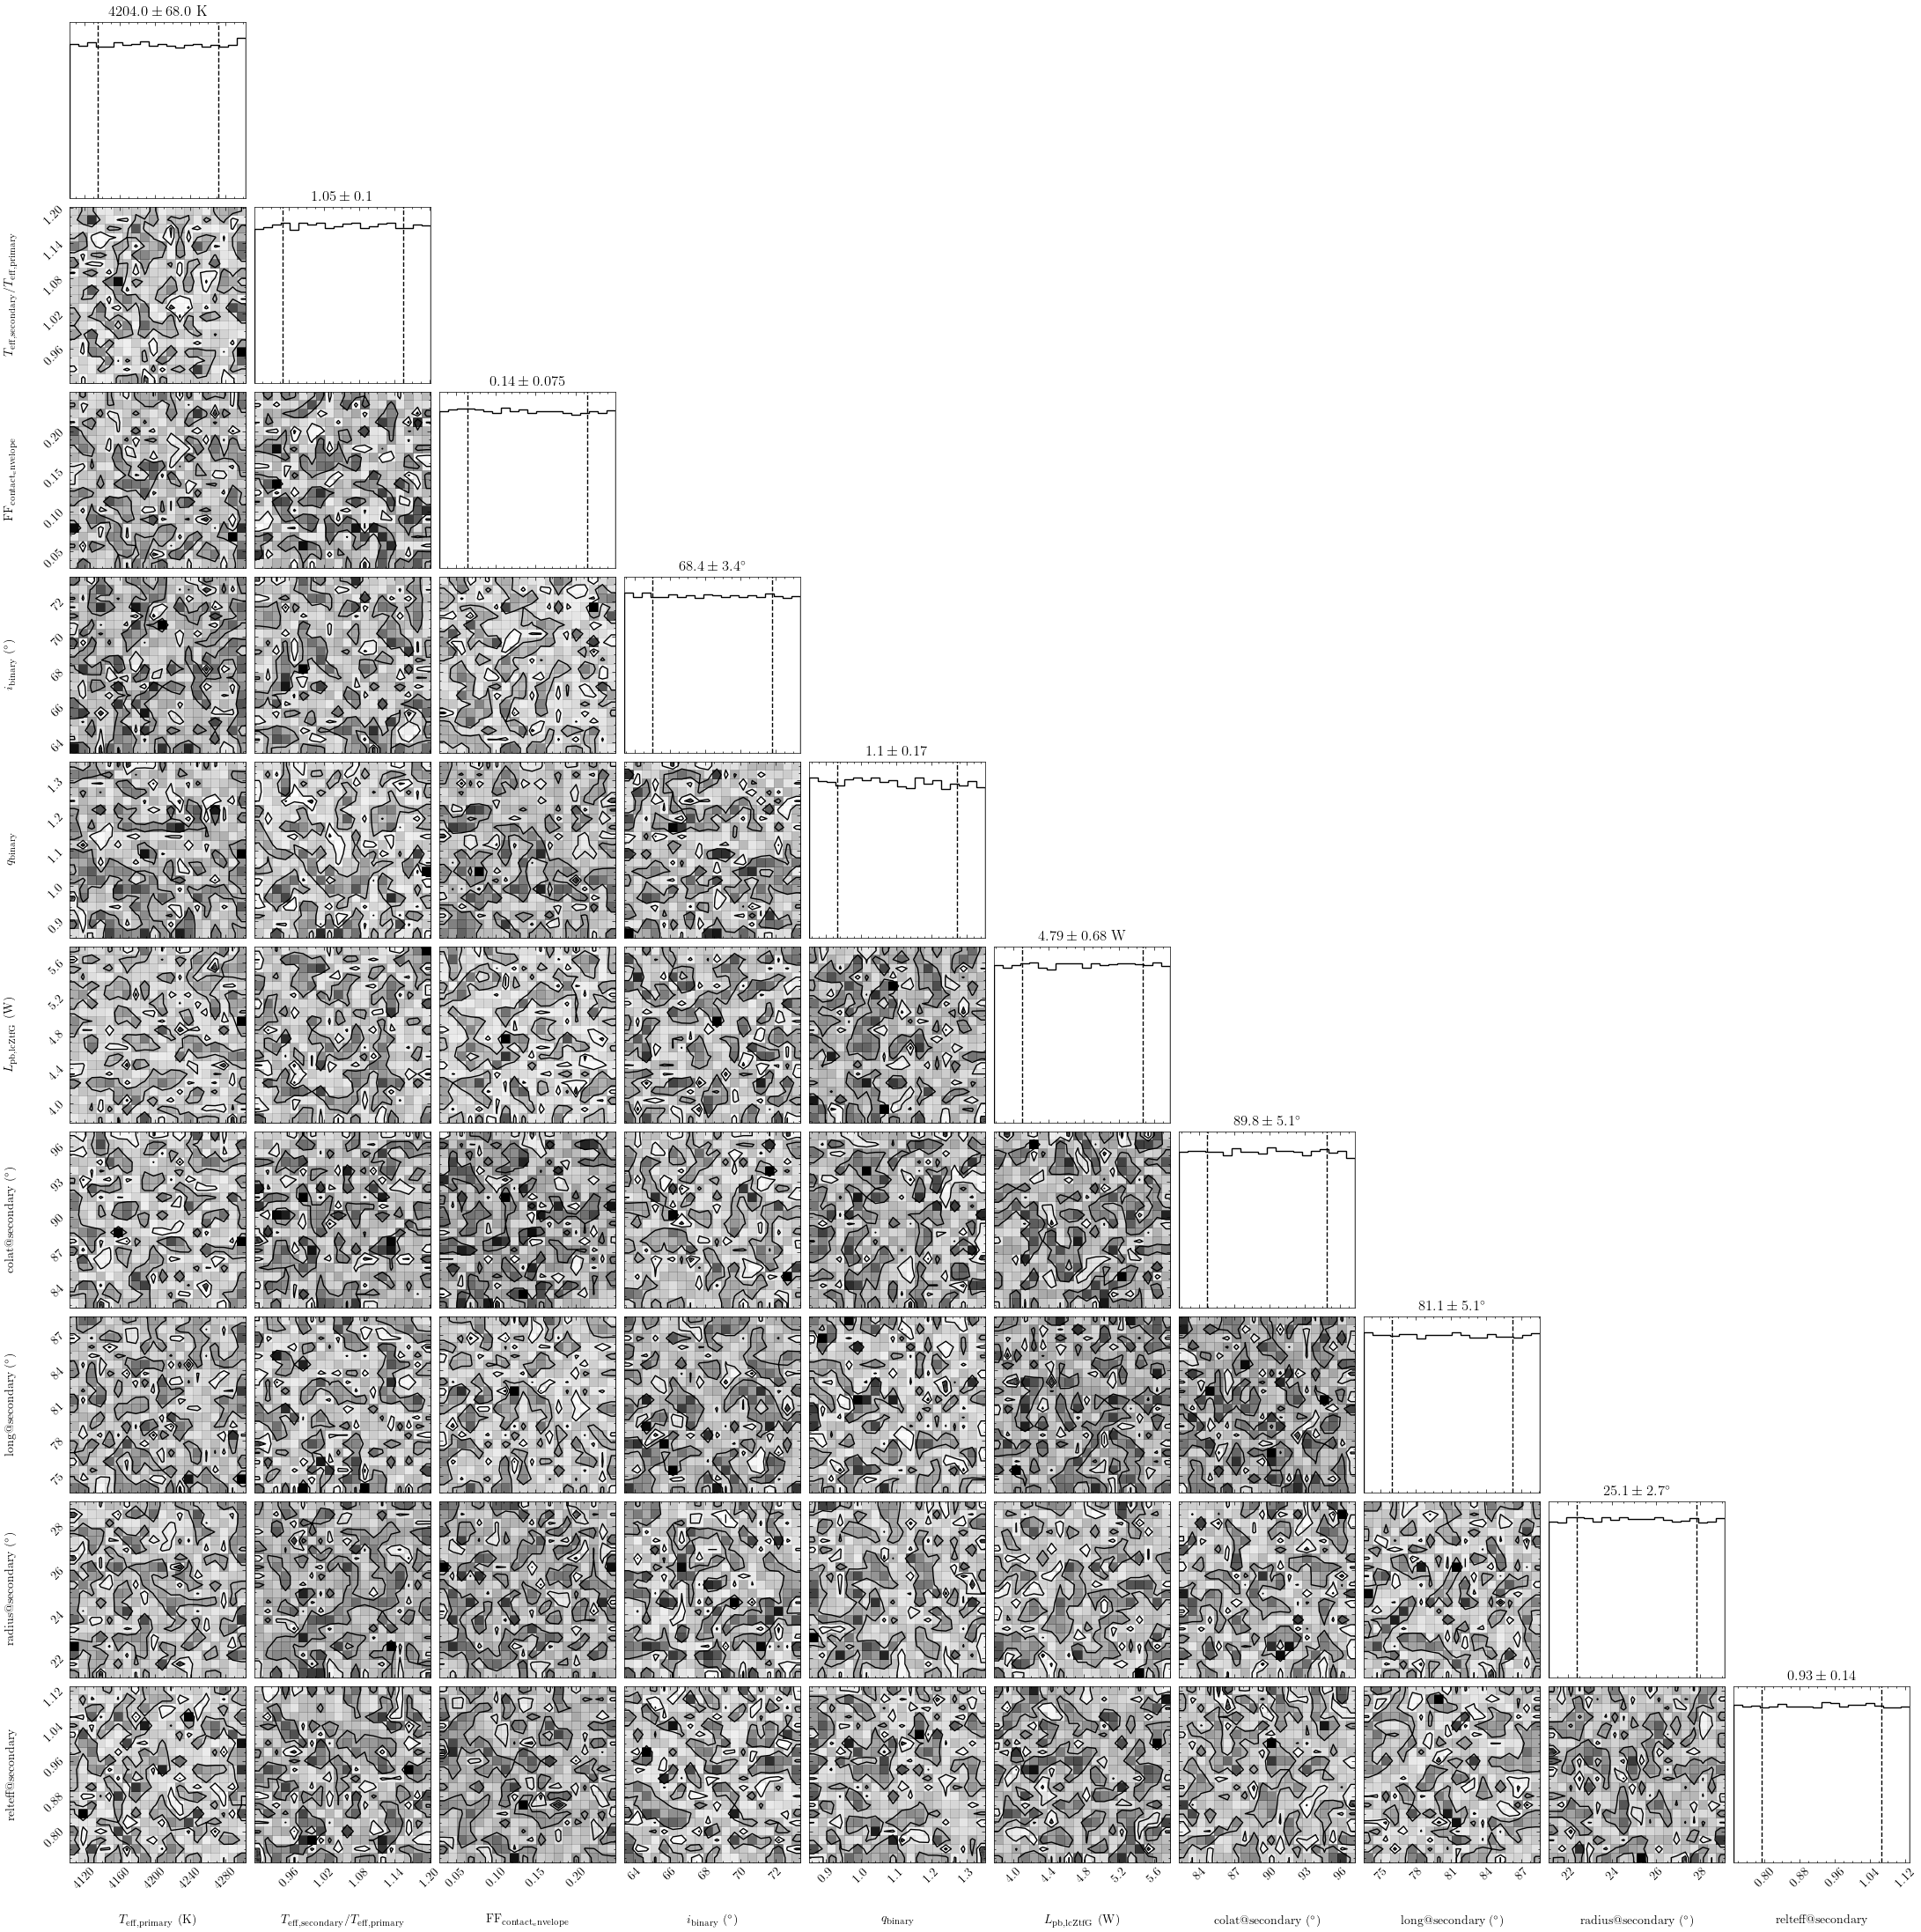
\includegraphics[scale=0.255]{Metodologia/Secciones/ModeloComputacional/Figures/Figura Prior Params Combinadas.png}
    \caption{Distribuciones uniformes de todos los parámetros muestreados
    utilizando cadenas de Monte Carlo (MCMC). La topología compleja que se ve en
    cada cuadrante se debe a las muestras que PHOEBE toma para cada parámetro en
    el proceso de generar la gráfica, no debido a la distribución almacenada por
    PHOEBE. Los priores, junto a esta gráfica, fueron generados en el Notebook
    \href{https://github.com/KnightIV/UANL_MAPTA_Observaciones/blob/main/analisis/phoebe_model/sampling/updated-data-mcmc-sampling.ipynb}{\code{updated-data-mcmc-sampling.ipynb}}.}
    \label{figuraPhoebePrioresCombinadasZtf}
\end{figure}

\section{Trazos Completos de los Caminadores} \label{apendice:modelo_computacional_graficas:trazos_completos_caminadores}

\begin{figure}[!ht]
    \centering
    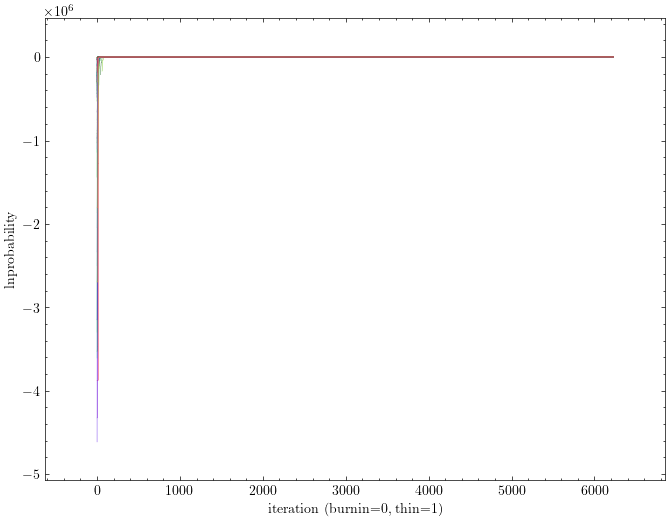
\includegraphics[scale=0.4]{Apendice/Figures/Figura Caminadores Trazo lnprobability 0 Burnin.png}
    \caption{Probabilidad logarítmica de cada caminador como función del número
    de iteraciones pasadas, después de 6233 iteraciones.}
\end{figure}

\begin{figure}[!ht]
    \centering
    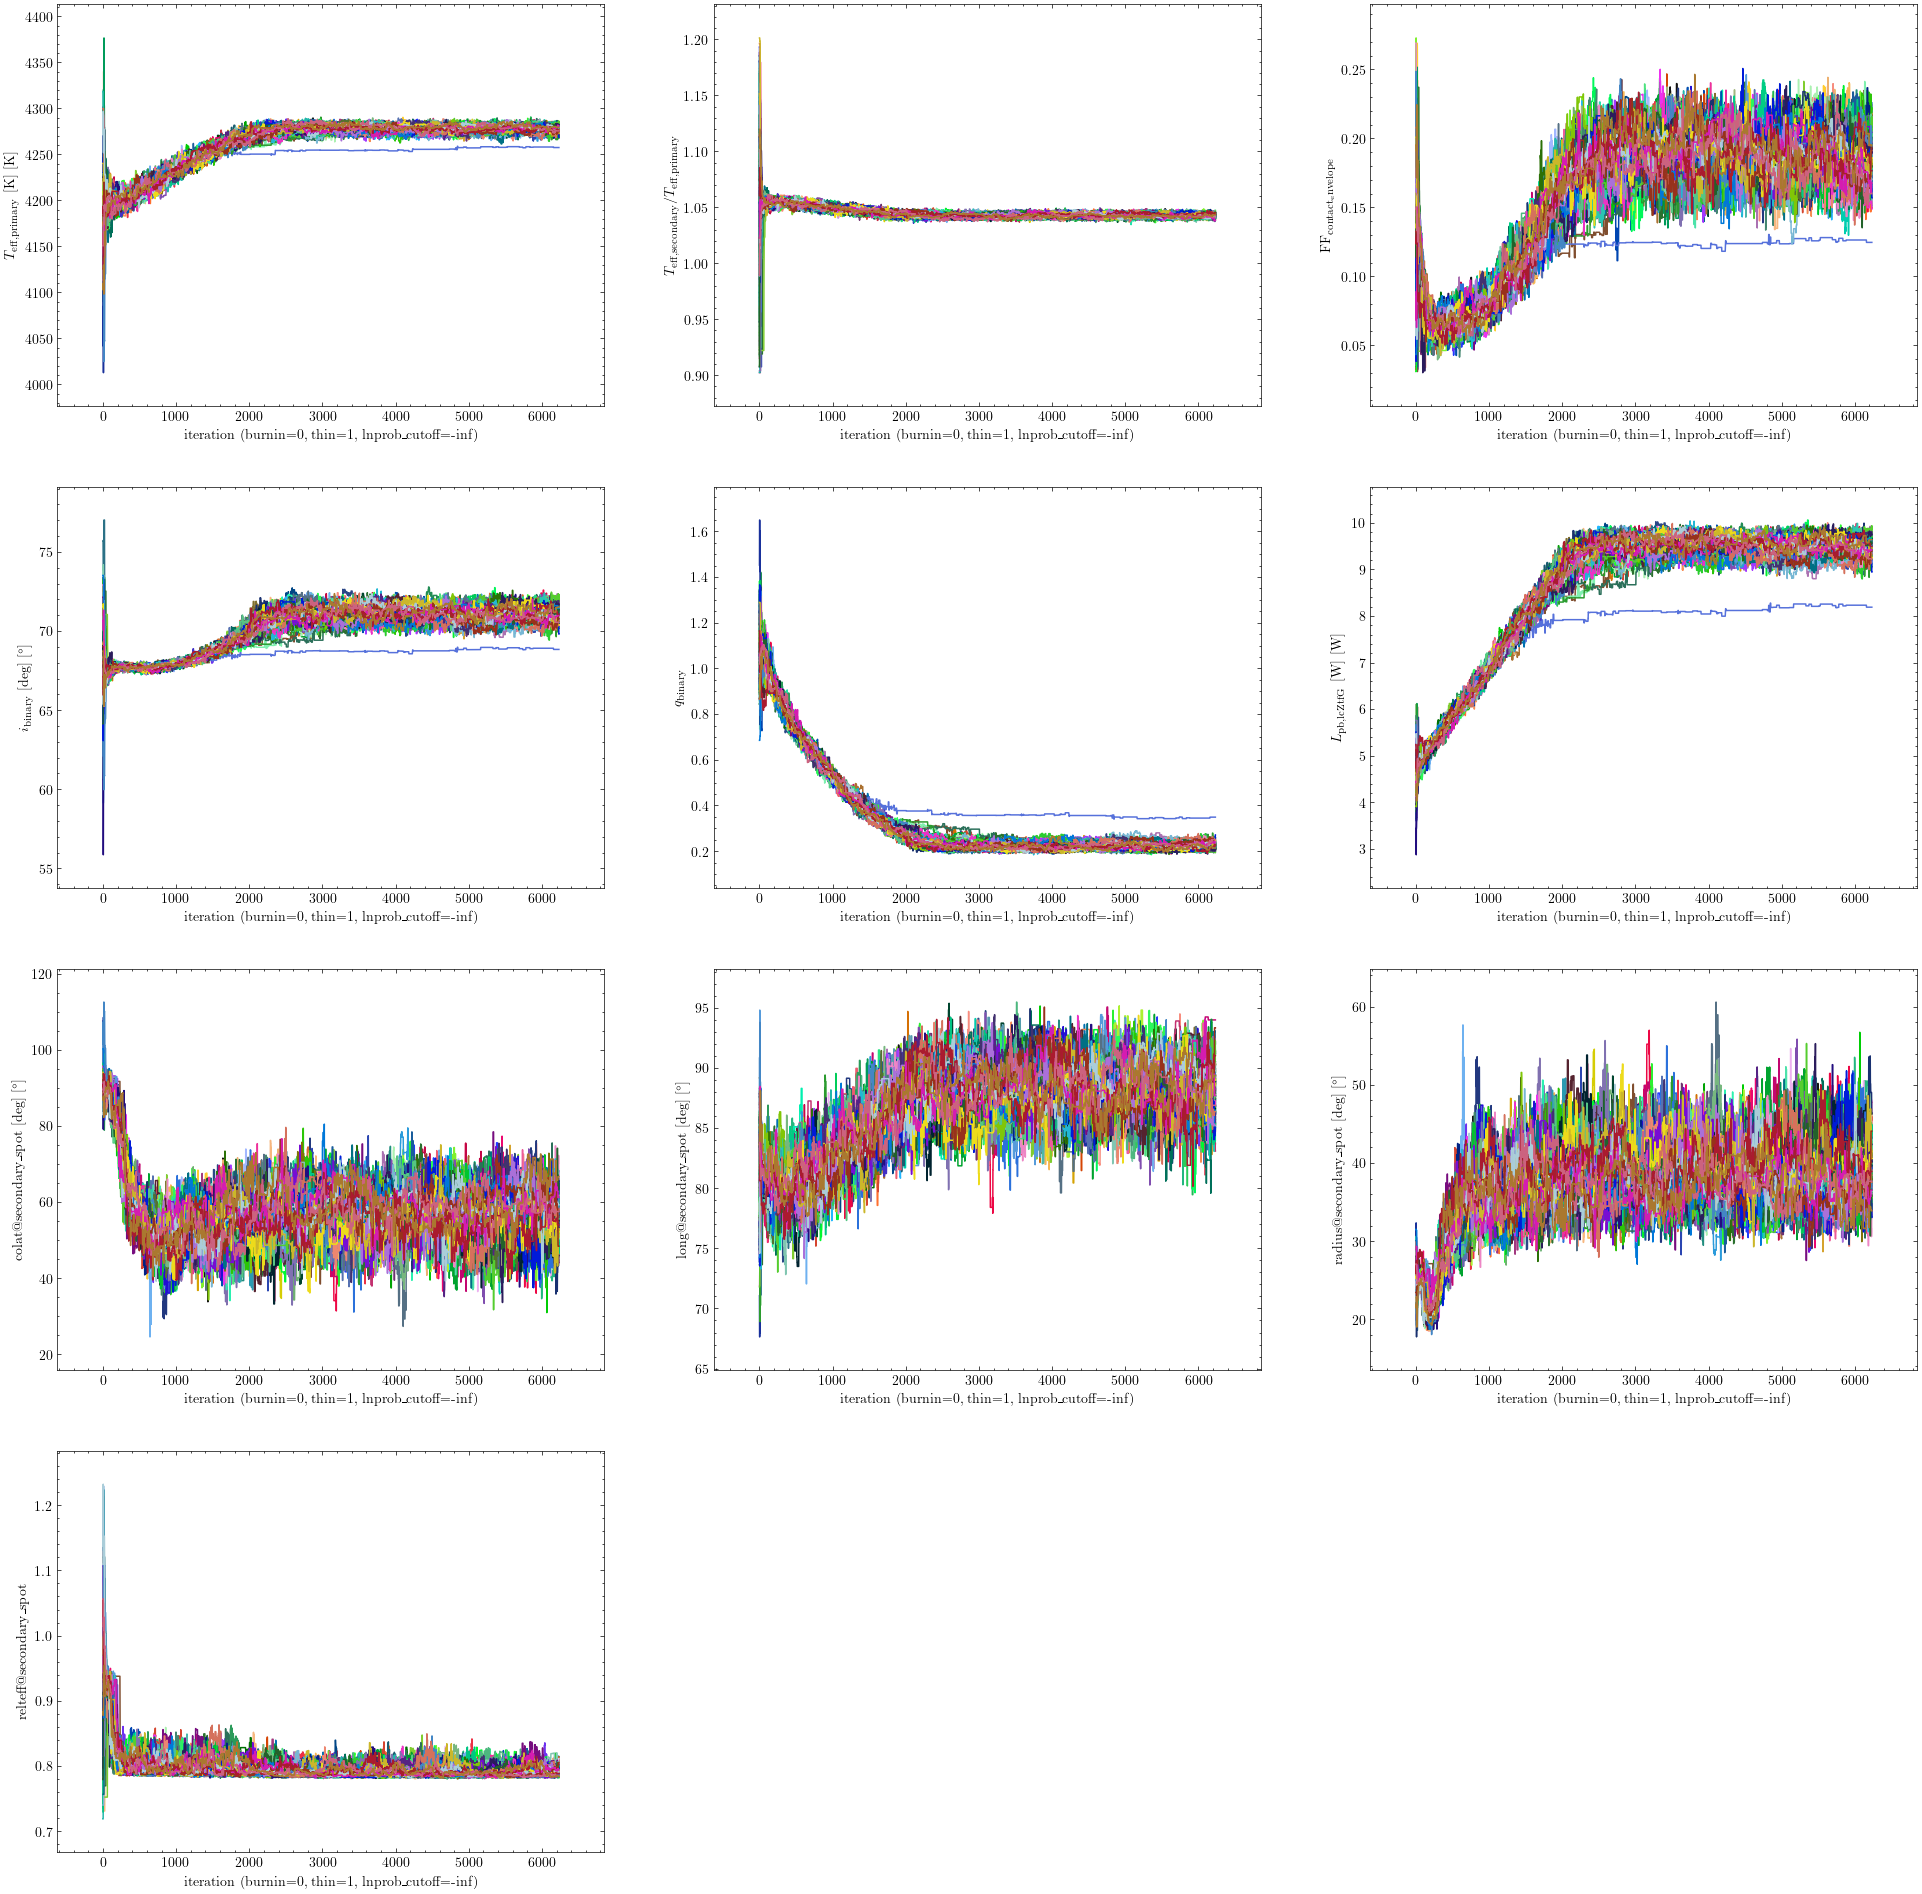
\includegraphics[scale=0.2]{Apendice/Figures/Figura Caminadores Trazo Parametros 0 Burnin.png}
    \caption{Valor de cada parámetro muestreado para todos los caminadores como
    función del número de iteraciones pasadas, después de 6233 iteraciones.}
\end{figure}

\section{Distribuciones de Densidad de Probabilidad Completas} \label{apendice:modelo_computacional_graficas:resultados_pdfs_completas}

\begin{figure}[!ht]
    \centering
    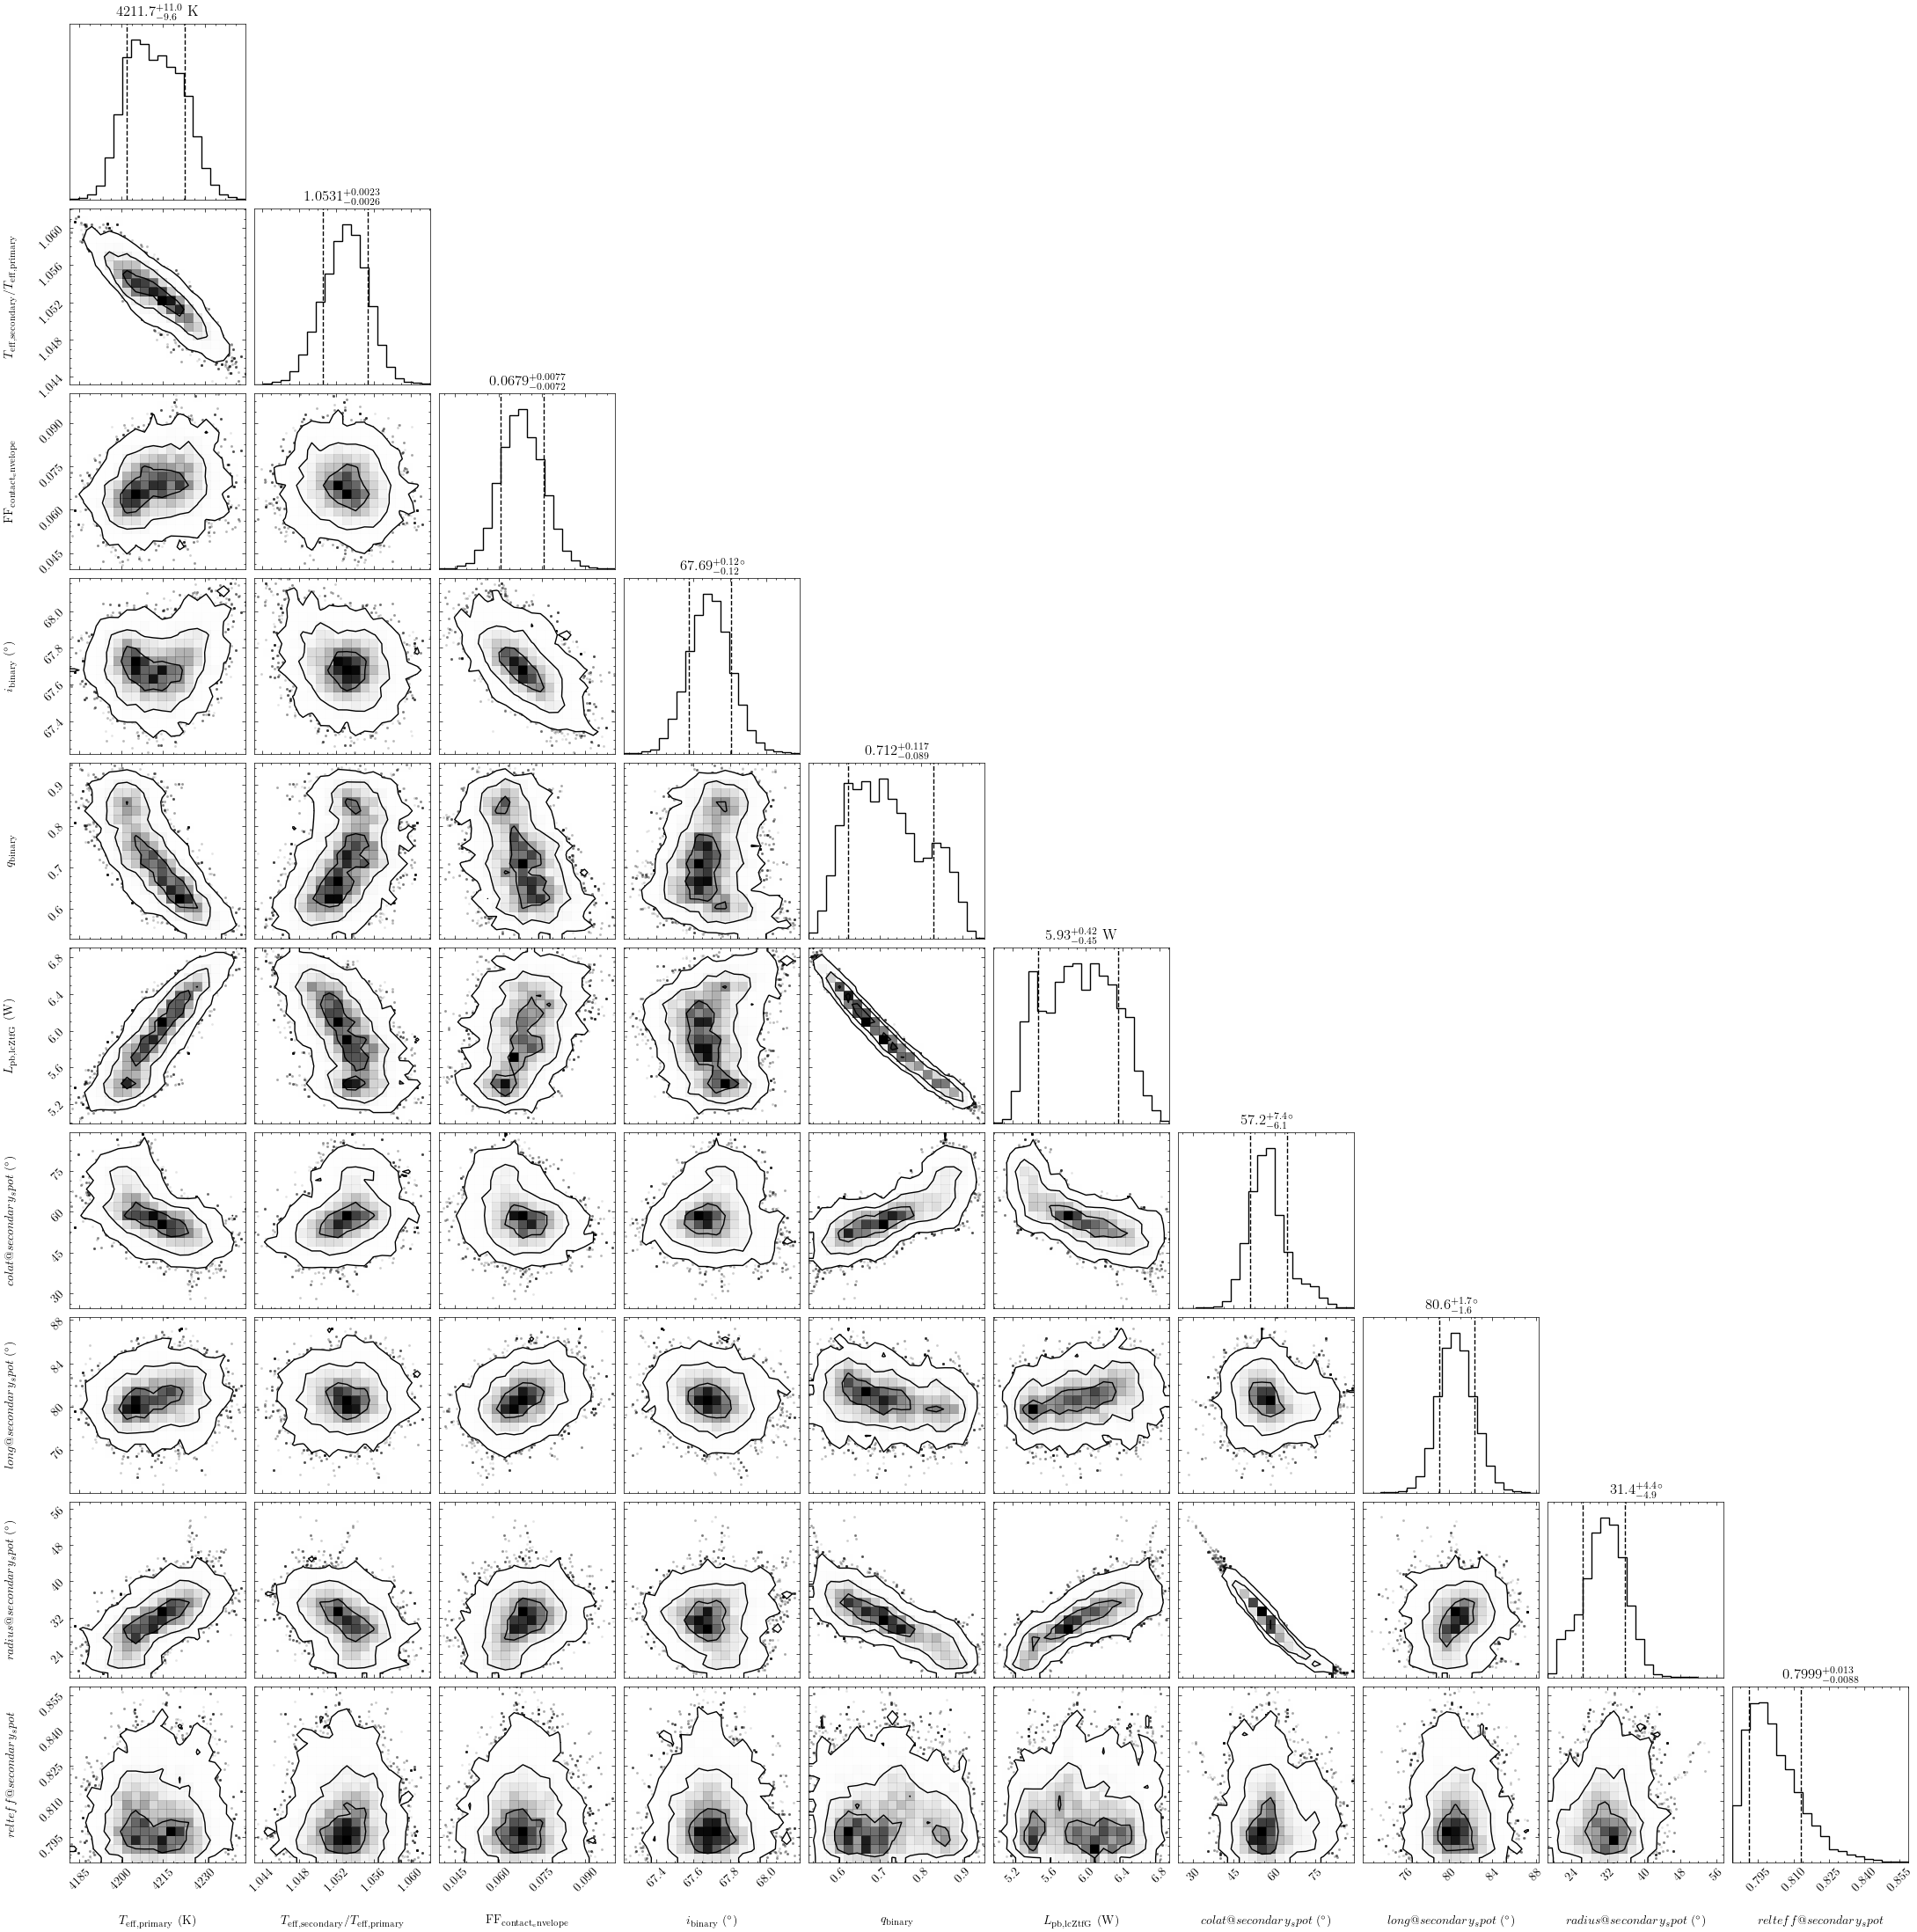
\includegraphics[scale=0.255]{Apendice/Figures/Figura MCMC ZTF Resultados Completos.png}
    \caption{Resultados completos del muestreo MCMC utilizando los datos de ZTF.
    Aquí se incluye el parámetro de molestia \code{pblum@primary@lcZtfG}, el
    cual representa la luminosidad en el pasabanda ZTF:g de la componente
    primaria, utilizada como el factor de escala para la curva de luz de ZTF:g y
    la temperatura efectiva del sistema reflejada por la curva de ZTF:r. Se
    puede apreciar la correlación lineal entre la razón de masa $q$ y la
    luminosidad de pasabanda.}
    \label{figuraPhoebeMcmcResultadosCompletos}
\end{figure}

\section{Correlaciones de Parámetros Muestreados} \label{apendice:modelo_computacional_graficas:correlaciones_parametros_muestreados}

\begin{figure}[!ht]
    \centering
    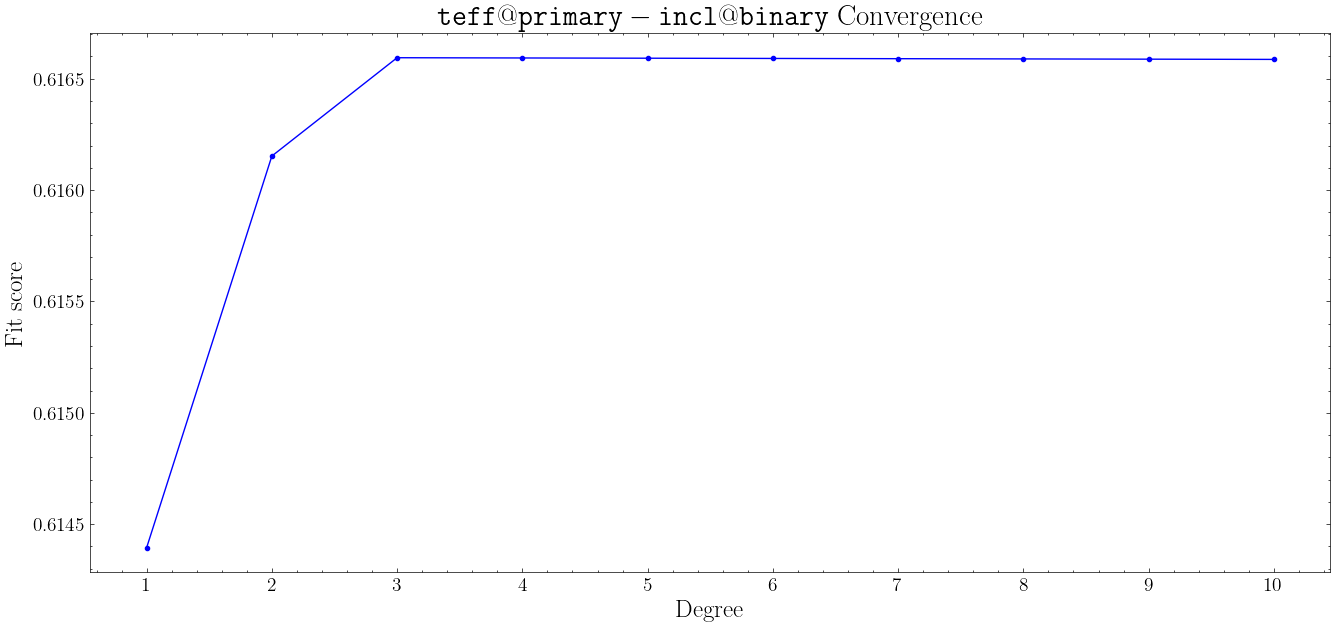
\includegraphics[scale=0.44]{Apendice/Figures/Figura incl-teff@primary Correlacion Convergencia.png}
    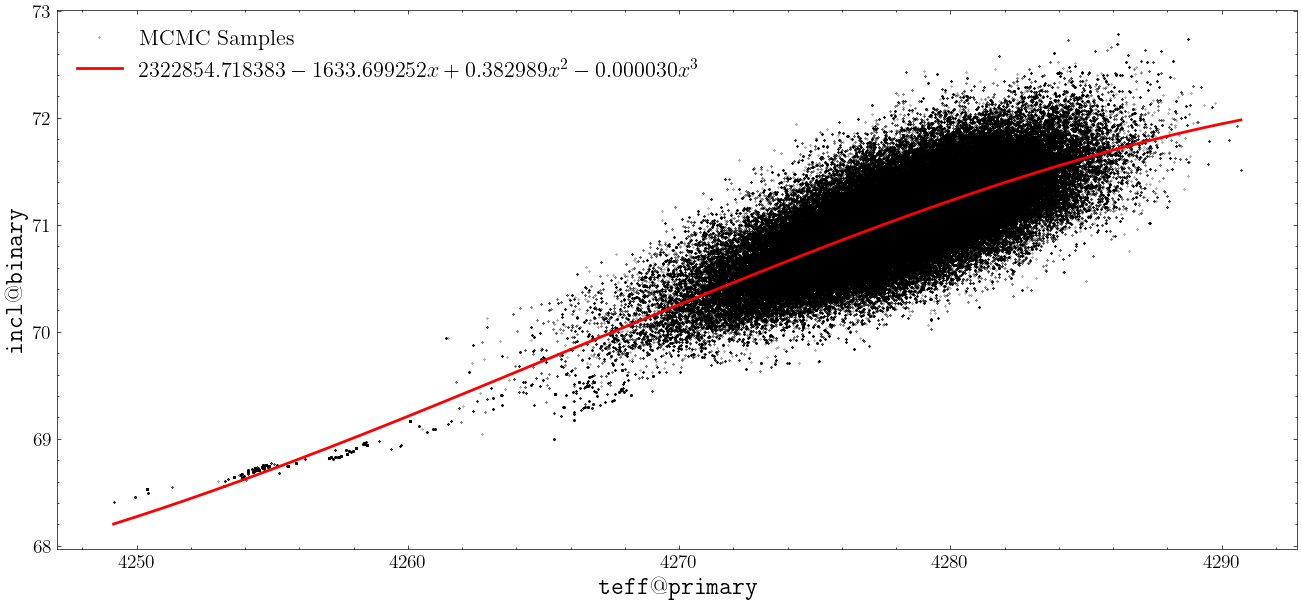
\includegraphics[scale=0.44]{Apendice/Figures/Figura incl-teff@primary Correlacion.png}
    \caption{Función polinomio ajustada a las muestras de la inclinación orbital
    \code{incl@binary} y la temperatura efectiva de la componente primaria
    \code{teff@primary}.}
\end{figure}

\begin{figure}[!ht]
    \centering
    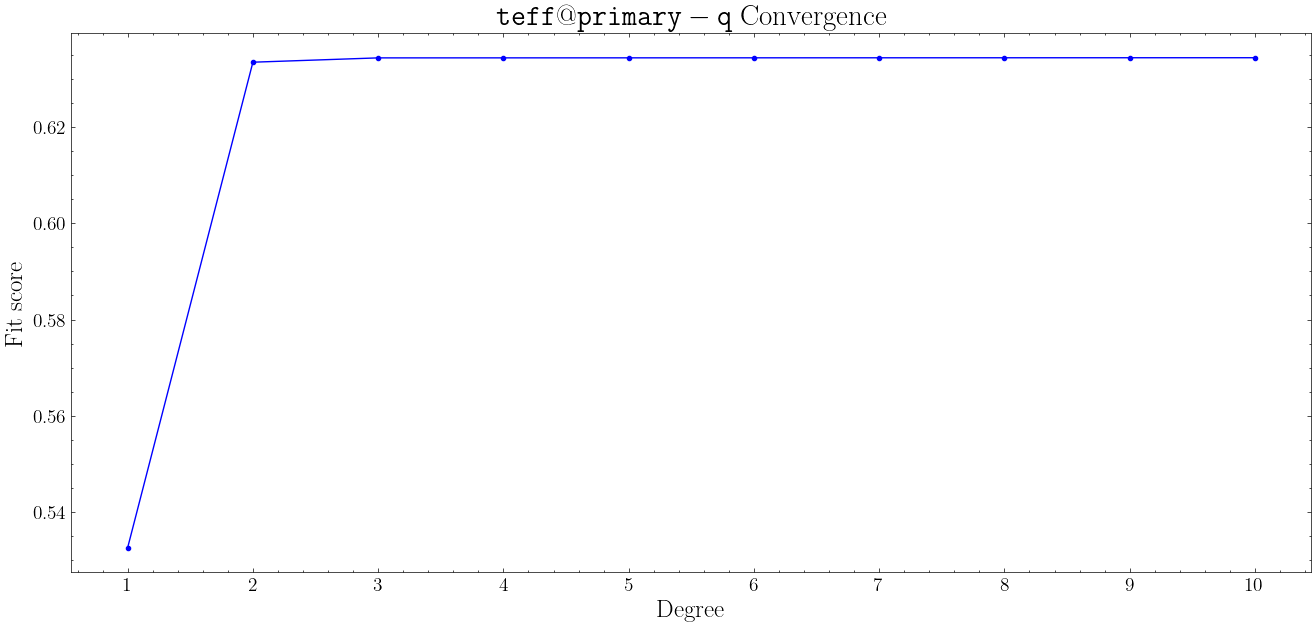
\includegraphics[scale=0.44]{Apendice/Figures/Figura q-teff@primary Correlacion Convergencia.png}
    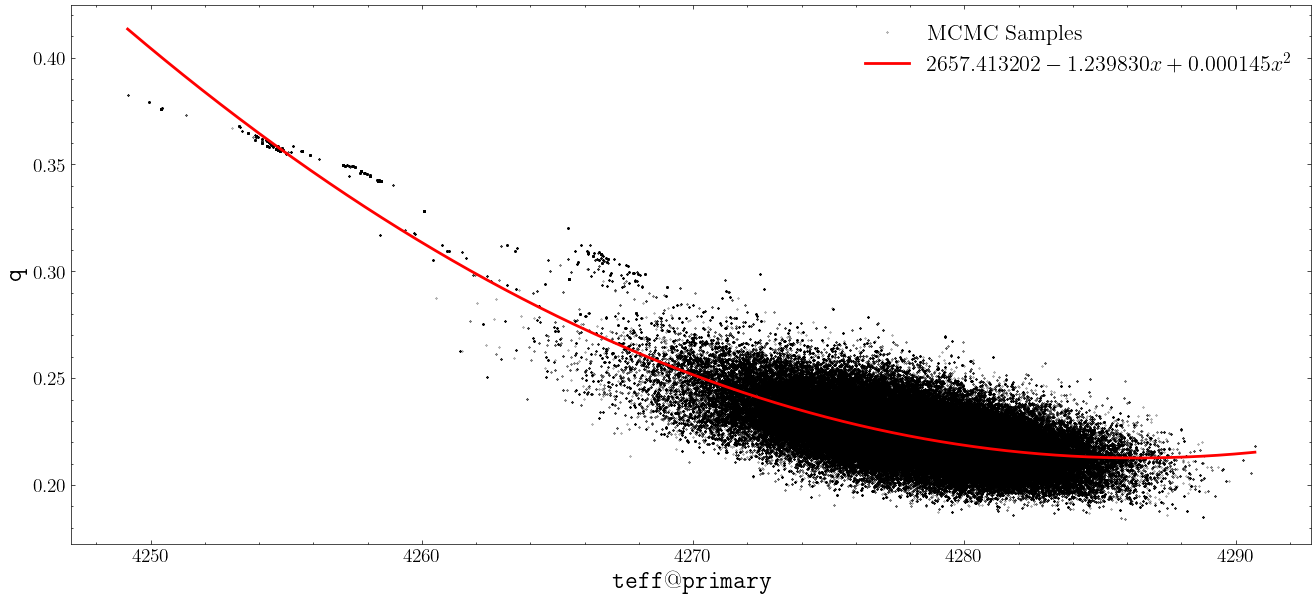
\includegraphics[scale=0.44]{Apendice/Figures/Figura q-teff@primary Correlacion.png}
    \caption{Función polinomio ajustada a las muestras de la razón de masa
    \code{q} y la temperatura efectiva de la componente primaria \code{teff@primary}.}
\end{figure}

\begin{figure}[!ht]
    \centering
    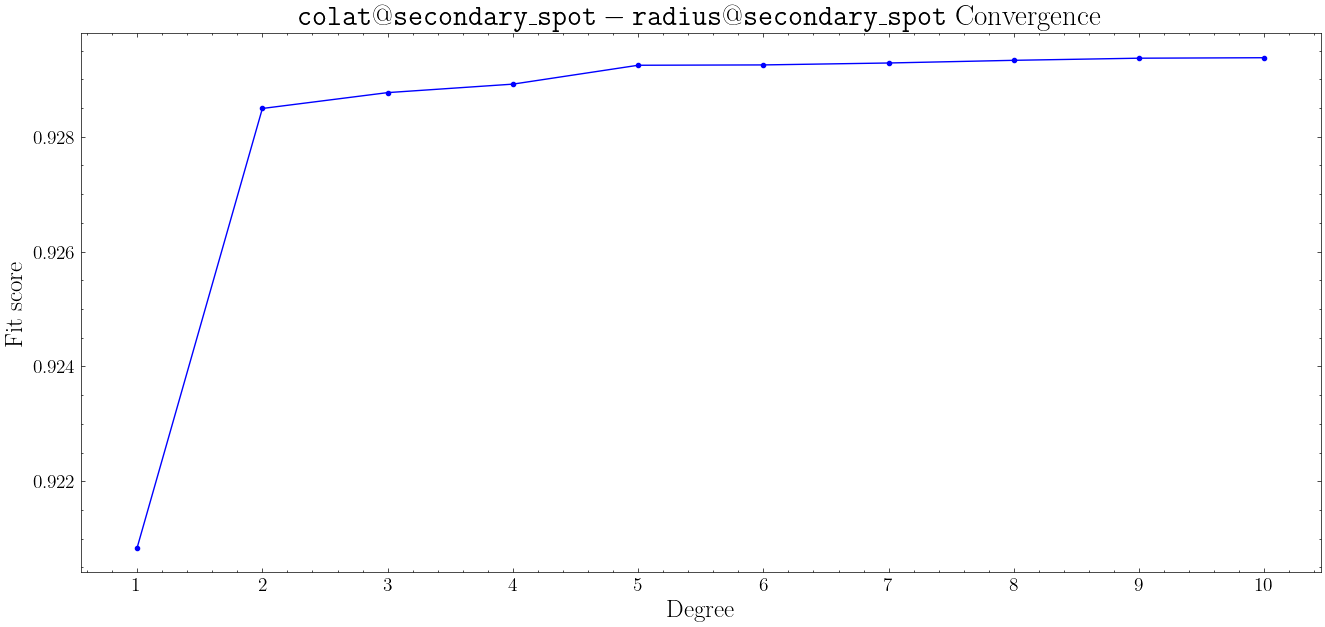
\includegraphics[scale=0.44]{Apendice/Figures/Figura radius@secondary_spot-colat@secondary_spot Correlacion Convergencia.png}
    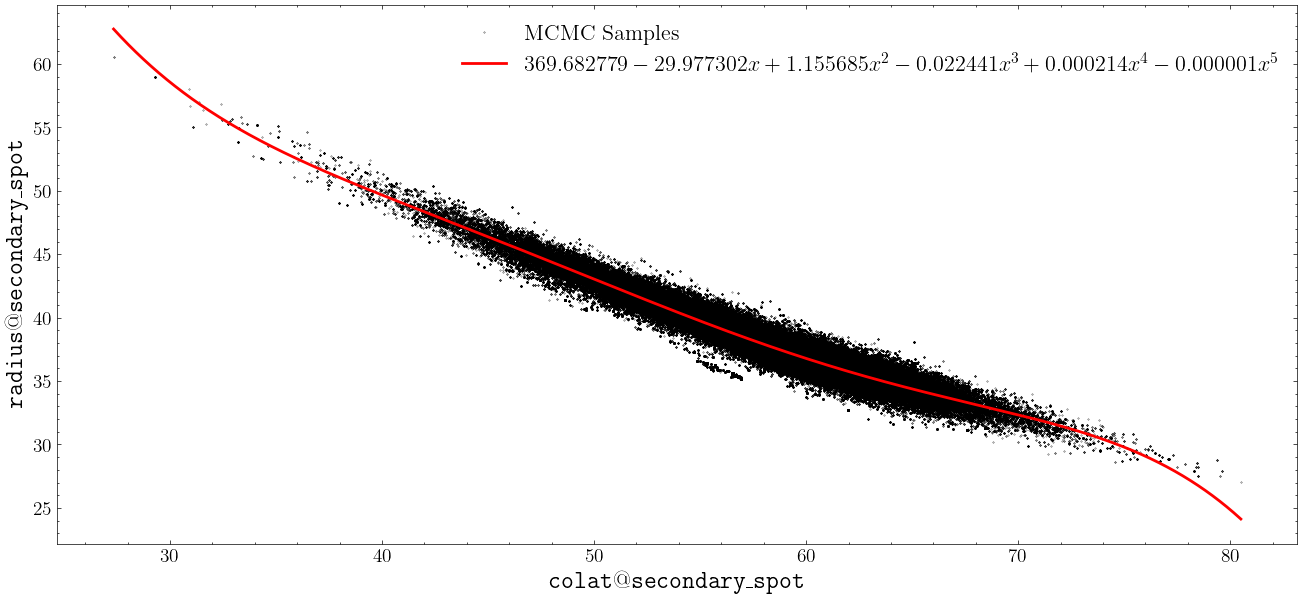
\includegraphics[scale=0.44]{Apendice/Figures/Figura radius@secondary_spot-colat@secondary_spot Correlacion.png}
    \caption{Función polinomio ajustada a las muestras del radio angular de la
    mancha en la superficie de la componente secundaria
    \code{radius@secondary\_spot} y su latitud \code{colat@secondary\_spot}.}
\end{figure}

\begin{figure}[!ht]
    \centering
    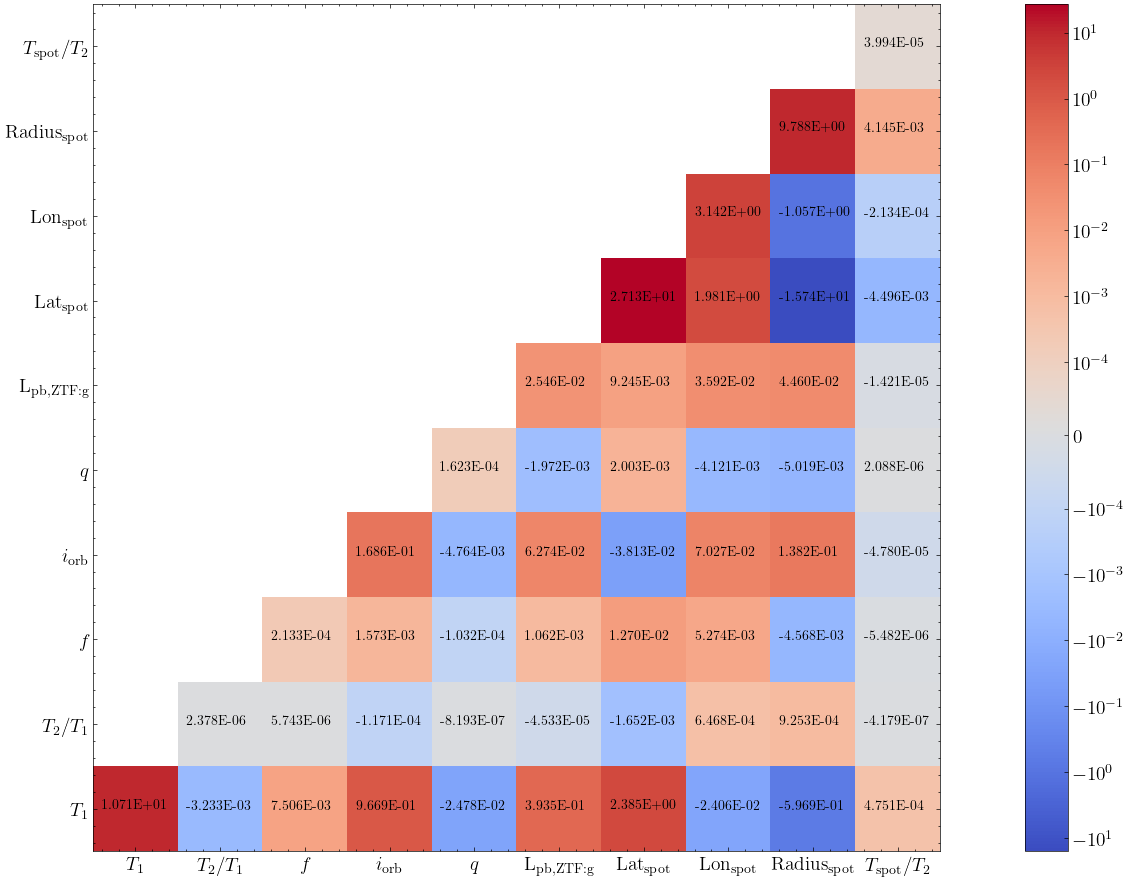
\includegraphics[width=1\linewidth]{Apendice/Figures/Figura ZTF MCMC Covarianzas.png}
    \caption{Matriz de covarianza entre los parámetros muestreados. Se muestra
    solo una diagonal por brevedad.}
    \label{figuraMcmcCovarianzas}
\end{figure}